\documentclass{article}
\usepackage[utf8]{inputenc}
\usepackage{indentfirst}
\usepackage[portrait, margin = 1in]{geometry}
\usepackage{array}
\usepackage{graphicx}
\usepackage{amsmath}
\usepackage{caption}
\usepackage{subcaption}
\usepackage{scicite}
\usepackage{textcomp}
\usepackage{siunitx}
\usepackage{hyperref}
\hypersetup{
    colorlinks=true,
    linkcolor=cyan,
    filecolor=magenta,      
    urlcolor=cyan,
    pdftitle={Probability and Statistics}
    }
\graphicspath{ {/home/brynn/Code/stats_mathreview/figures} }


\title{Probability and Statistics}
\author{Brynnydd Hamilton}
\date{August 17, 2022}

\begin{document}
\tableofcontents

\maketitle

\section{Introduction/Philosophy}
Many people have taken classes in probability and statistics, but I always found those terms very vague. What are probability and statistics, and what's the difference between them?

Probability theory is what we use to understand the \textbf{likelihood of random events}. It tells us how we can manipulate probabilities of different events. As applied scientists (i.e., not mathematicians), we don't \textit{really} think about probability theory that much, we're more concerned about describing the characteristics of our dataset through statistics.

However, having a good understanding of probability theory is essential to understanding statistics, since all statistics are just applications of probability theory. If statistics is painting, probability is perspective and color theory. It's the underlying mechanics of statistics. You can kind of think of probability as more cut-and-dry (there is usually a ``right'' answer, as opposed to in statistics, where there are better and worse ways to do things, but no ``right'' answers).

I really like that metaphor, because, much like many people can look at the same scene and paint different pictures of it, there are infinite ways to use statistics in your research to analyze your dataset. Every choice that you make in experiment setup, data processing, and analytical techniques will have an impact on your resultant statistics. That can be overwhelming, but it's a key thing to keep in your head at all times. And it's also important to keep in mind that statistics is always a simplification, so you will always be ``losing'' information. However, we have to lose some information to come up with an understandable system. 

``Whenever you're dealing with a model or with a situation, there are zillions of details in that situation. And when you come up with a model, you choose some of those details that you keep in your model, and some that you say, well, these are irrelevant'' - John Tsitsiklis

\section{Probability}

\subsection{How to Talk about Probability}
When people want to talk about probability theory, they will often work with random variables denoted by a capital letter, commonly an $X$ or $Y$. Technically speaking, a random variable is something called a \textit{measurable function}, which is a function between two sets in two measurable spaces, one of which is a probability space, that preserves the structure of the space. It's important to note that these can be discrete (our output is a finite set) or continuous (our output is a number anywhere within some range, an infinite set).

Oftentimes there can be many ways to describe a sample space, for the same process (e.g. flipping a coin: one sample space is {heads, tails}, another sample space is {heads, tails and it's raining, tails and it's not raining}). Note that the way we define a sample space will guide our interpretation of the problem. Therefore, it's important to think about having the right ``granularity'' in your definition of your sample space for a specific problem. 

We refer to a \textbf{event} as some subset of the sample space.

We assign probability to our events, with a probability between 0 (not gonna happen!) and 1 (absolutely gonna happen!). We will use the notation that $\mathbf{P}(A)$ is the probability that event $A$ occurs. 

Some axioms of probability are... 
\begin{enumerate}
\item\label{item:2} nonnegativity
\item normalization (probability of entire sample space = 1)
\item additivity

If two events do not intersect
\begin{equation}
\label{eq:3}
A \cap B = 0 %don't overlap
\end{equation}
Then the union of the two events is equal to the sum of their independent probabilites
\begin{equation}
\label{eq:2}
P(A \cup B) = P(A) + P(B) %add up
%this implies that probability <= 1 
\end{equation}
\end{enumerate}

When defining a sample space, we want the events of the sample space to have the following characteristics 
\begin{enumerate}
\item\label{item:1} mutually exclusive
\item collectively exhaustive 
\end{enumerate}

For a sample space, we will define a ``probability law'', which tells us how probability is distributed in the sample space. We can use probability laws to analyze a random variable. These can come from physics or data.

If you take a probability class, you'll spend hours playing around with these statistics. I'm going to focus on some applications of conditional probability, because I think that's one of the more relevant avenues of probability theory. Conditional probability is how we incorporate our prior knowledge of a situation into our estimate of probability. 

\subsection{Conditional Probability}
We define the notation $\mathbf{P}(A|B)$ as the probability of A, given that B occurred.
\begin{equation}
\label{eq:6}
\mathbf{P}(A|B) = \frac{\mathbf{P}(A \cap B)}{\mathbf{P}(B)}
\end{equation}
A consequence of this definition is what we call the \textbf{Joint Probability}
\begin{equation}
\label{eq:7}
\text{Joint Probability: }\mathbf{P}(A \cap B) = \mathbf{P}(B) \mathbf{P} (A|B)
\end{equation}
and because an intersection is order-invariant, we can also say 
\begin{equation}
\label{eq:11}
\mathbf{P}(A \cap B) = \mathbf{P}(A) \mathbf{P} (B|A)
\end{equation}

\subsubsection{Independence}
One concept that impacts a lot of calculations is \textbf{independence}, which tells us if two probability distributions are related to one another.

If an event $A$ is \textbf{independent} from event $B$, then $\mathbf{P}(A|B) = \mathbf{P}(A)$. For our earlier example where we defined our sample space as follows
\begin{equation}
\label{eq:5}
S =
\begin{cases}
  \text{heads} \\
  \text{tails and its raining} \\
  \text{tails and its not raining}
\end{cases}
\end{equation}
we would find that $\mathbf{P}(\text{tails}|\text{raining}) = \mathbf{P}(\text{tails})$, indicating that the probability of rain is independent from the probability of our coin landing on tails.

\subsubsection{Example: False Alarms}
See the attached .ipynb with a Julia example of this situation

Imagine we have a piece of equipment that detects whales. We know that for our region of study, there are whales there 5\% of the time.
\begin{equation}
\label{eq:8}
\mathbf{P} = 
\begin{cases}
  0.95 & \text{no whale} \\
  0.05 & \text{whale}
 \end{cases}
\end{equation}

Furthermore, our equipment will detect the whale 99\% of the time \textbf{if there is a whale there} (if we miss a whale: Type II error, false negative). It will detect a whale 10\% of the time \textbf{if there is no whale there} (if we detect a whale: Type I error, false positive).

If we get a detection signal, what's the probability that it's actually a whale?
Hint: calculate
\begin{equation}
\label{eq:10}
\mathbf{P}(\text{whale} | \text{detection}) = \frac{\mathbf{P} (\text{whale} \cap \text{detection})}{\mathbf{P}(\text{detection})}
\end{equation}
% answer: P (whale \cap detection) = P(whale) * P(detection | whale) = 0.05 * 0.99
% answer: P(detection) = 0.05 * 0.99 + 0.95 * 0.1
% answer: P(whale | detection) = 0.34

\subsubsection{Bayes Theorem/Law/Rule}
This example helps show the power of what's called Bayes Theorem/Law/Rule (depending on who you ask - and there's a lot of strong opinions about it!). We can use it to incorporate prior information into our analysis. Specifically, Bayes' theorem is  used to incorporate prior knowledge about the situation into the estimate of the probability of an event, $A_i$. A formal definition of it is given in Equation \ref{eq:9}. 
\begin{equation}
\label{eq:9}
\text{Bayes' Theorem: }\mathbf{P} (A_i|B) ==\frac{\mathbf{P}(A_i)\mathbf{P}(B|A_i)}{\mathbf{P}(B)}
\end{equation}
An intuitive way to think about this theorem is that it takes the probability of both events occurring, and divides it by the normalizing factor. 
There is a whole field of analysis surrounding this fundamental idea called \textbf{Bayesian Analysis}. If you want to see a good example of using Bayesian analysis, check out this \href{https://github.com/christopherpiecuch/bevir}{Github repo from Chris Piecuch}.

\section{Statistics}
\subsection{Probability Density Functions}
Statistics is what we we use whenever we want to think about analyzing and making decisions about a dataset. In statistics, we'll be working with \textbf{probability density functions} (PDFs) and \textbf{cumulative distribution functions.}. Although we think about PDFS more often, it can be easier to think about the CDF first.

We will define a CDF with a capital $P$, and it will be defined for the random variable $x$ as $P_x()$. CDFs are defined such that $P_x(X)$ is the probability that $x \leq X$. At $-\infty$, the CDF is 0, and at $+\infty$, the CDF is 1. You can interpret the CDF as the probability that a value is equal to or less than $X$. It is the integral of all the probabilities up to that point. 

We will define a PDF with a lowercase $p$ and will be defined similarly to the CDF, $p_x()$. The PDF is the derivative of the CDF and is normalized so that its integral over all $X$ is 1. You can interpret the CDF of as the probability of $X$ occurring. 

An example of the PDF and CDF are shown in Figure \ref{fig:pdfvcdf} for the Normal distribution.

\begin{figure}[htbp]
\centerline{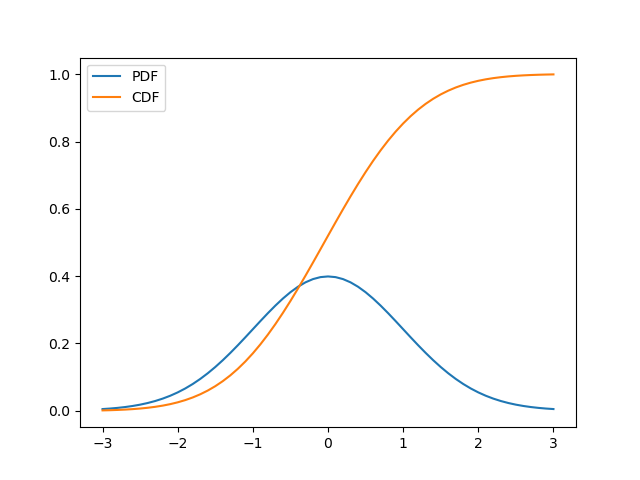
\includegraphics[width = 0.75\textwidth]{pdfvcdf.png}}
\caption[]{\label{fig:pdfvcdf} The normal distribution as a PDF and CDF.}
\end{figure}

\subsection{Statistics for Understanding Distributions}
\subsubsection{Ways to Describe One Distribution}
Two terms we'll use all the time to talk about distributions are the \textbf{mean} and \textbf{variance}.

The mean is also referred to as the first moment, average, or expectation value. One way to think about it is that it is the ``center of mass'' of the distribution.

The variance helps us define the ``spread'' of the distribution, or how far we vary away from the mean, on average.

In Table \ref{table:1}, I show the mathematical definitions for mean and variance, for continuous and discrete cases. The continuous case is what we use when we talk about functions defined for all real numbers. However, when we are dealing with real data, we will usually use the discrete definition. Note that the definition of variance will change if we are talking about ``sample'' or ``population'' variances. 

\begin{table}[h!]
  \centering
  \begin{tabular}{|c||c|c|}
    
    \hline
    & Continuous & Discrete \\
    \hline
    Mean $<x>, \mu$ & $\int^\infty_\infty X p_x(X)dX$ & $\frac{\sum_i^N x_i}{N}$ \\[0.75ex] 
    \hline
    Variance $<(<x-<x>)^2>$ & $\int^{\infty}_{-\infty}(X - <x>)^2 p_x(X) dX$ & $\frac{\sum_i^{N} (x_i-\bar{x})^2}{N}$\\[0.75ex]
    \hline
  \end{tabular}
  
  \caption{The continuous and discrete definitions of the mean and variance.}
  \label{table:1}
\end{table}

We also will frequently talk about \textbf{standard deviation, which is the square root of variance}, and another measure of the spread of a distribution.

One further question we can ask is ``how does the variance vary?'' This is equivalent to asking about the asymmetry of the the distribution or the \textbf{skewness}. The skewness comes from the idea of standardized moments (it's the 3rd standardized moment), and is defined as such
\begin{equation}
\label{eq:12}
\text{Skewness: } <\left(\frac{X - \mu_XX}{\sigma_XX}\right)^{3}>
\end{equation}
You can take this one step further, and look at the 4th standardized moment (i.e., raise the quantity in Equation \ref{eq:12} to 4), we will have a measure of the ``tailedness'' of the distribution, called \textbf{kurtosis}.

Finally, you may recall talking about quartiles and quantiles in your previous statistic classes. A quantile is the more general definition, and it can be considered the cut point of a probability distribution into continuous intervals with the same probability. We can have a quantile for any percentage. The 25\% quantile is the first quartile, and it is the point where 25\% of the data lies ``below''. The 50\% quantile is the median, and 75\% quartile is the third quantiles. The space between the first and third quartiles is referred to as the interquartile range. 

It is important to be cognizant of how extreme values (sometimes outliers) will affect these statistics. For a statistic like ``range'' (the difference between the maximum and minimum values of the dataset), it will be heavily impacted by extreme values. Mean and variance will be more impacted by extreme values than the median and interquartile range. 

For discrete sets, we can also look at the following statistics
\begin{itemize}
\item median: for the ordered dataset, the middle value (similar to mean, less impacted by extreme values)
\item mode: the most common value (not really used a lot, tells us something about frequency)
\end{itemize}

\subsubsection{Ways to Talk About Two Distributions}
If we are dealing with two distributions, we can ask if they are related to each other by looking at the correlation (how they are related) or the covariance (how they differ). I show these definitions in Equations \ref{eq:1} and \ref{eq:4}, where $\mu_Z$ denotes the mean of random variable $Z$ and $\sigma_Z$ denotes the standard deviation, and $<Z>$ represents taking the mean of whatever is between the brackets.

\begin{equation}
\label{eq:1}
\text{Covariance: } <\left(X - \mu_X \right) \left( Y - \mu_Y \right) >
\end{equation}
\begin{equation}
\label{eq:4}
\text{Correlation: } \frac{ <\left(X - \mu_X \right) \left( Y - \mu_Y \right) >}{\sigma_X\sigma_Y}
\end{equation}

As we see in the above equations, correlation is a scaled covariance. Sometimes you will hear it referred to as a Pearson correlation coefficient, of which there are a few mathematical definitions. It is also sometimes referred to as an r-value. Pearson correlation is most sensitive to linear relationships, and there are other measures of correlation that are more sensitive to nonlinear relationships. As correlations are not scaled, you should not compare correlation coefficients between datasets.

Covariance, which is correlation scaled by standard deviation, ranges from -1 to +1, with -1 indicating perfect anticorrelation, 0 indicating independence, and +1 indicating perfect correlation. Covariance can be compared between datasets. 


\subsection{Distribution Statistic Example: Average Daily Air Temperatures in Florida}
Now, we will do an example applying these statistical measures we've defined. We will look at daily average air temperatures from three different locations in Florida: St Petersburg, Tampa Bay, and Fort Myers. In Figure \ref{fig:florida}, I plot the three locations of the datasets. A common, and frequently overlooked, part of data analysis is to think about the physics (or what you already know) of the problem before you begin. What do you expect to see?

Some things I would expect to see is the coastal effect (cooler temperatures near the coast) as well as the urban effect (warmer temperatures in urban areas). What would you expect to see in terms of variability? Extreme values? 

\begin{figure}[htbp]
\centerline{\includegraphics[width = 0.5\textwidth]{/home/brynn/Pictures/florida2.png}}
\caption[]{\label{fig:florida}The locations of our three datasets.}
\end{figure}


The next, and still sometimes overlooked, step in data analysis is to make some exploratory graphs of your data to get a feel for its form. Since this is time-series data, I plot it with respect to day. You should be able to get an idea for the mean, variance, extreme values, and correlation from this plot. I also plot a histogram to get a better sense of the  distribution (mean value, variance, extreme values) with all temporal aspects removed.

\begin{figure}[htbp]
\centerline{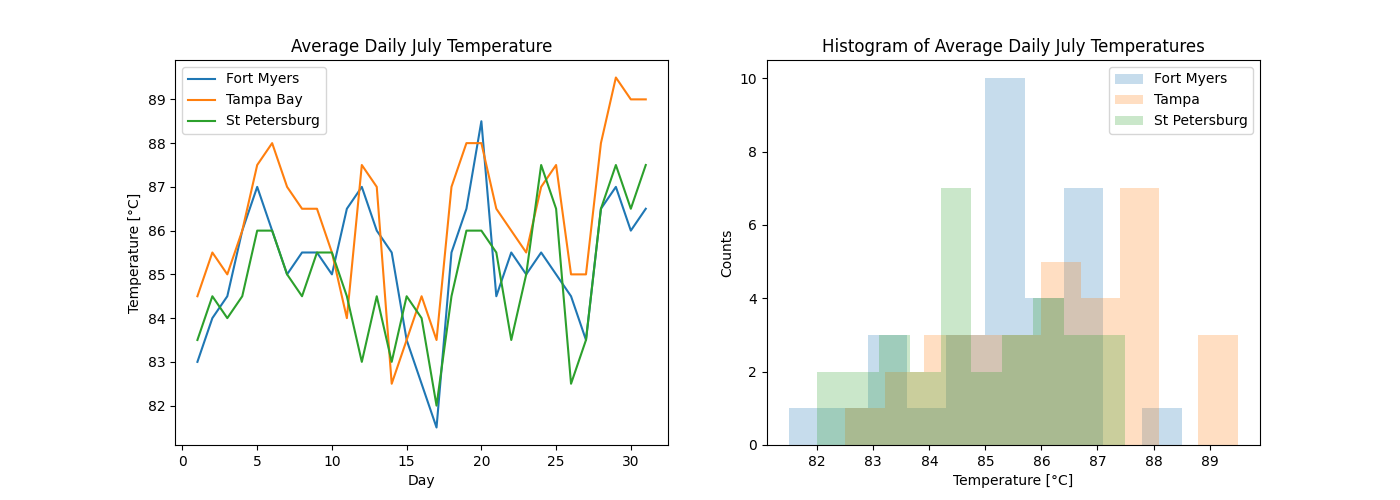
\includegraphics[width = \textwidth]{distex.png}}
\caption[]{\label{fig:ex} On left, data plotted as timeseries. On right, data plotted as a histogram. }
\end{figure}

I think two great tenets of data analysis are
\begin{enumerate}
\item Have an idea of what you'd expect every time you \textbf{calculate} or \textbf{visualize} anything
\item\label{item:5} Plot everything, in multiple ways. 
\end{enumerate}

In the accompanying Jupyter Notebook, I walk through several ways to visualize this dataset. I think it's really important, whenever you're dealing with multiple datasets, to visualize everything together, as well as on its own axes. This really helps to highlights comparative features (i.e., ``this mean is higher than that mean'') as well as stand-alone features (i.e. ``this dataset has some really large extreme values in comparison to the rest of it'').

I also walk through calculating all the statistics we previously discuss, and come up with an interpretation of this dataset.

\subsection{Normal Distribution and the Central Limit Theorem}
``Normally distributed'' is a phrase that you'll hear a lot in statistics. The Normal Distribution, also referred to as the Gaussian (pronounced ``gau-see-an'') Distribution (or the bell-curve) refers to a distribution that takes the form

\begin{equation}
\label{eq:13}
f(x) = \frac{1}{\sigma\sqrt{2\pi}}e^{-\frac{1}{2} \left( \frac{x - \mu}{\sigma} \right)^{2}}
\end{equation}

\clearpage
Normal distributions are important because of two interrelated reasons
\begin{enumerate}
\item\label{item:3} Central Limit Theorem
\item Many statistical techniques apply only to normally distributed variables
\end{enumerate}

What's the Central Limit Theorem? The Central Limit Theorem states that, for any random variable, with any distribution, the fluctuations between it's sample mean and population mean will become normally distributed, when scaled by the number of samples. It can be a little difficult to grasp the magnitude of this theorem, so I present it, step by step here. 

First, let's assume we have some weird distribution, like a gamma distribution. This distribution is always positive, has its highest value at 0, and trails off from there. Definitely not a normal distribution! I show this in Figure \ref{fig:gamma}
\begin{figure}[htbp]
\centerline{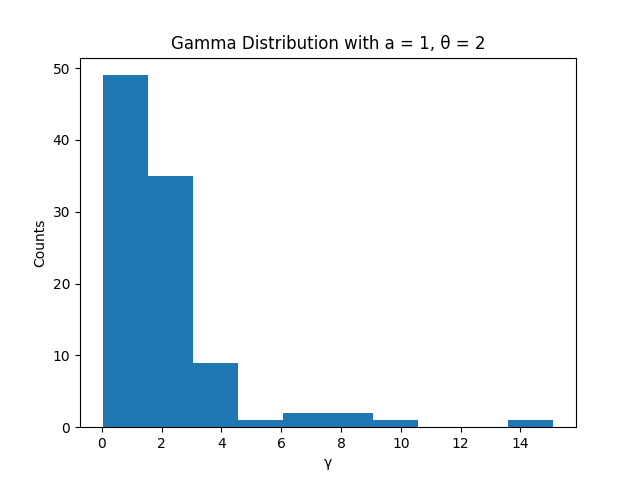
\includegraphics[width = 0.5\textwidth]{gamma.png}}
\caption[]{\label{fig:gamma} Histogram of 100 points taken from Gamma distribution}
\end{figure}

The law of large numbers says that, as we take progressively larger samples, the mean of any distribution will probably converge. For posterity, I demonstrate this in Figure \ref{fig:lawoflarge}, where I take progressively larger samples from our gamma distribution and calculate the mean.
\begin{figure}[htbp]
\centerline{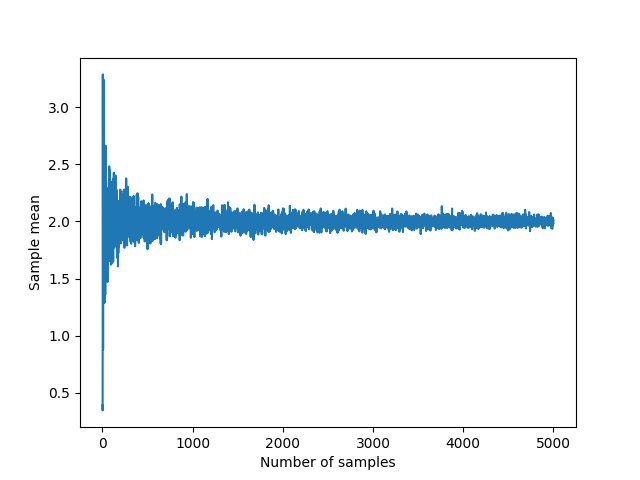
\includegraphics[width = 0.5\textwidth]{lawoflarge.png}}
\caption[]{\label{fig:lawoflarge} Demonstration of law of large numbers}
\end{figure}
In Figure \ref{fig:lawoflarge}, we see that there is a lot of oscillation for smaller sample sizes ($<1000$), and then it seems like our sample mean settles around 2 (but there is still some noise!).

We'll take the mean for some very large sample size and call this our population mean. Next, for progressively larger number of sample sizes, we'll calculate the following scaled fluctuation metric
\begin{equation}
\label{eq:14}
f(n) = \sqrt(n)(\mu_{x_n} - \mu_{x})
\end{equation}
where $n$ is the number of samples, $\mu_{x_n}$ is the mean of a $n$ samples taken from our random distribution, and $\mu_x$ is our population mean (the horizontal asymptote of Figure \ref{fig:lawoflarge}.

In Figure \ref{fig:clt}, I show the result of taking histograms of the distribution of values calculated by taking progressively larger samples. We see that it approaches the normal distribution!

\begin{figure}[htbp]
\centerline{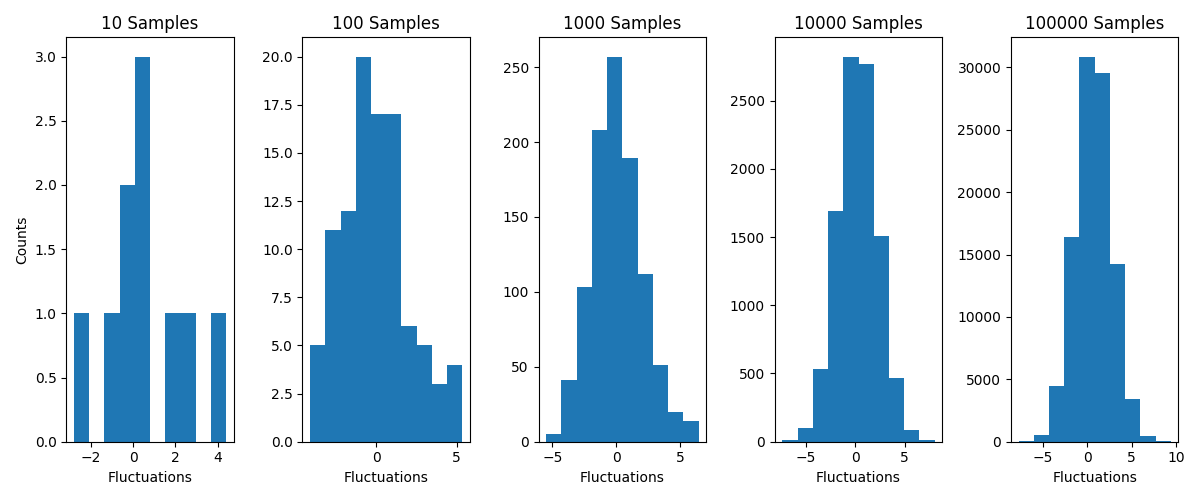
\includegraphics[width = \textwidth]{clt.png}}
\caption[]{\label{fig:clt} }
\end{figure}

\subsection{Hypothesis Testing}
An important question in statistics is whether your results are significant. The boundary for significance is very field-dependent, but oftentimes people will use the idea of the null hypothesis and a t-test to prove significance. Here is the protocol for this
\begin{enumerate}
\item\label{item:4} Formulate a \textbf{null hypothesis} and a \textbf{alternative hypothesis}. Usually your null hypothesis is that your data has no significance, and your alternative hypothesis is that it does. For my temperature example, I might make the following hypotheses.

  \textbf{Null Hypothesis}: Average temperature in Tampa Bay is less than \textbf{or equal to} $85^{\circ}$C in June.

  \textbf{Alternative Hypothesis}: Average temperature in Tampa Bay is greater than $85^{\circ}$C in June.

  Note: your null hypothesis should always have the ``equals'' because it suggests that this is the most conservative estimate that your null hypothesis could satisfy.
  
\item Determine the appropriate test statistic. This depends on your alternative hypothesis $H_a$

\begin{itemize}
\item if $H_a:\mu>\mu_0$: upper-tailed test
\item if $H_a:\mu<\mu_0$: lower-tailed test
\item $H_a:\mu\neq\mu_0$: two-tailed test
\end{itemize}


Examples of test statistics include z-tests (commonly used in teaching because its a little easier to understand, but not as applicable for research because we don't always know the population $\sigma$) and t-tests. Below, I show the equation for a t-test, one of the more commonly used tests (note the connection to the Central Limit Theorem here: our data doesn't need to be normally distributed, because were looking at the differences between population and sample mean, which we now know is normally distributed!). 

\begin{equation}
\label{eq:15}
t = \frac{\bar{x}-\mu_0}{\sigma / \sqrt{n}}
\end{equation}

\item Calculate $t$, and then map it on to a Student's t-distribution. Compute the probability, or p-value, by integrating to the extrema. Compare this to your level of significance (commonly, you want p $< 0.05$ to reject the null hypothesis).
  
\end{enumerate}  
You will very rarely see this process laid out in papers. Oftentimes, people will just report the p-value. 

\subsection{Linear Regression}
Another basic statistical technique is finding the trend in data. There are several ways to do this, but linear regression is one of the most basic and common. It can be a great starting point to inform future analysis. A common way to do this is linear least squares, which  minimizes the distance between each datapoint and the regression line. There are several ways to represent this calculation, but I'm going to show it with linear algebra. As you progress to more advanced statistics, most things are represented with linear algebra, so this is a good introduction to thinking about your statistics in terms of vectors and matrices. 

Linear regression assumes that we have an independent variable $x$ and a dependent variable $y$ and that they are linearly related, so we can assume a relationship of the following form for every data point 

\begin{equation}
\label{eq:16}
y = m x + b
\end{equation}

In Eq. \ref{eq:16}, $m$ is a constant that is the slope, or trend (how much does change in $y$ does a change in $x$ elicit). $b$ is a constant that is the y-intercept, or offset. Here, $x$ and $y$ are our knowns, and we want to solve for $m$ and $b$. Is there a way we can rephrase this well-known equation so it's purely linear algebra (i.e., we want to put those coefficients into a vector)?

Well, adding a coefficient in an equation like we do with $b$ in Eq. \ref{eq:16} is the same thing as adding a vector of ones multiplied by the coefficent in linear algebra, like so
\begin{equation}
\label{eq:17}
\vec{y} = m \vec{x} + b \vec{1}
\end{equation}
And remember, when we multiply a matrix by a vector, we're essentially multiplying the first value in the vector by the first column, multiplying the second value in the vector by the second column, and so forth, and then adding all resultant columns together. So we can rewrite Eq. \ref{eq:17} like
\begin{equation}
\label{eq:18}
\vec{y} = \mathbf{E} \vec{c}
\end{equation}
$\mathbf{E}$ in Eq. \ref{eq:17} is the horizontal concatenation of the one-vector and the $\vec{x}$ vector, like so
\begin{equation}
\label{eq:19}
\mathbf{E} =
\begin{bmatrix}
  x_1 && 1 \\
  x_2 && 1 \\
  \dots && \dots \\
  x_n && 1 \\
\end{bmatrix}
\end{equation}
and $\vec{c}$ in Eq. \ref{eq:17} is the coefficient vector, like so
\begin{equation}
\label{eq:20}
\vec{c} =
\begin{bmatrix}
  m \\
  b \\
\end{bmatrix}
\end{equation}
We'll now define something called the noise vector, or the misfit vector, which is the error incurred by assuming values for $m$ and $b$. This noise vector $n$ is defined as such
\begin{equation}
\label{eq:21}
\vec{n} =  \vec{y}-\mathbf{E} \vec{c}
\end{equation}
Now, the vector $\vec{n}$ will tell us the mismatch between every data point and its value as calculated according to our coefficent vector $\vec{c}$. We want to minimize the magnitude of this vector. We can calculate a vector's magnitude by multiplying its transpose by itself, like so
\begin{equation}
\label{eq:22}
J = \vec{n}^T\vec{n}
\end{equation}
This is equivalent to squaring every element of the noise vector and adding all the values together to create a scalar. Now, we want to minimize this scalar. The best way to do this is to take the derivative of $J$ with respect to the coefficent vector $\vec{c}$ and set it equal to zero. Recall how our scalar $J$ depends on $\mathbf{E}, \vec{y}$ and $\vec{c}$
\begin{equation}
\label{eq:23}
J = (\vec{y} - \mathbf{E}\vec{c})^T(\vec{y} - \mathbf{E} \vec{c})
\end{equation}
By the chain rule for linear algebra, 
\begin{equation}
\label{eq:24}
\frac{\partial J}{\partial \vec{c}} = \frac{\partial \vec{n}}{\partial \vec{c}} \frac{\partial J}{\partial \vec{n}}
\end{equation}
Now we calculate the derivative of the noise vector with repsect to the coefficient vector, finding
\begin{equation}
\label{eq:25}
\frac{\partial\vec{n}}{\partial \vec{c}} = \frac{\partial (\vec{y} - \mathbf{E} \vec{c})}{\partial \vec{c}} = -\mathbf{E}^{T}
\end{equation}
Now, we calculate the derivative of the scalar $J$ with respect to the noise vector, finding
\begin{equation}
\label{eq:26}
\frac{\partial J}{\partial \vec{n}} = \frac{\partial (\vec{n}^T\vec{n})}{\partial \vec{n}} = 2 \vec{n} = 2(\vec{y}-\mathbf{E}\vec{c})
\end{equation}
Now we can multiply together the results of Eqs. \ref{eq:25} and \ref{eq:26}, finding that
\begin{equation}
\label{eq:27}
\frac{\partial J}{\partial \vec{c}} = -2 \mathbf{E}^T \vec{n} = -2 \mathbf{E}^T (\vec{y} - \mathbf{E}\vec{c})
\end{equation}
Now, recall that the scalar $J$ will be minimized when this derivative is equal to zero. So now we can solve for our coefficent vector $\vec{c}$.
\begin{equation}
\label{eq:28}
0 = -2 \mathbf{E}^T (\vec{y} - \mathbf{E}\vec{c}) = \mathbf{E}^T (\vec{y} - \mathbf{E}\vec{c})
\end{equation}
\begin{equation}
\label{eq:29}
\mathbf{E}^T \vec{y} =  \mathbf{E}^T \mathbf{E}\vec{c}
\end{equation}
In linear algebra, we take the inverse instead of multiplying, so
\begin{equation}
\label{eq:30}
( \mathbf{E}^T \mathbf{E} ) ^{-1} \mathbf{E}^T \vec{y} = \vec{c}
\end{equation}

Although the calculus might be a little less intuitive, solving this via linear algebra can make it much easier to extend this calculation to propagate error, and it makes the relation clearer for higher order regression. It also is very fast and computationally efficient.

Let's quickly calculate the trend of our Tampa Bay temperature dataset. I show this calculation in the attached Jupyter Notebooks. In one very short, efficient line of code, I calculate both the slope and y-intercept in one fell swoop. Here's the result

\begin{figure}[htbp]
\centerline{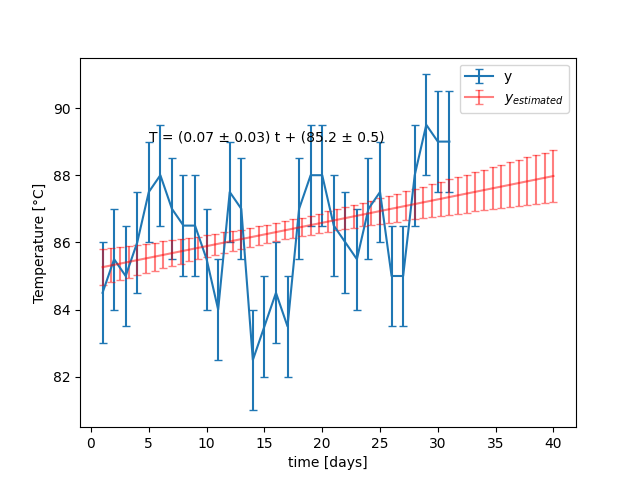
\includegraphics[width = 0.75\textwidth]{regression.png}}
\caption[]{\label{fig:regression} Result of computing the linear regression of for the June average daily temperatures in Tampa Bay}
\end{figure}

\section{Conclusion}
This was a cursory introduction to many of the basics of statistics. The techniques outlined here are good for assessing the basics of your datasets, but will essentially never be enough on their own. Reading literature in your field is one of the best ways to understand what common statistical techniques are and see how their used. It can also help you understand what appropriate data pre-processing practices are.

\clearpage
\section{Acknowledgements}
This review builds on materials from prior math review courses, taught by
\begin{itemize}
\item Arianna Krinos
\item The 2019 Instructor Who Didn't Write Their Name on Their Notes
\item Jeffrey Mei
\item Hannah Mark
\end{itemize}

It also builds on
\begin{itemize}
\item class notes from 12.805 (Data Analysis in Physical Oceanography, taught by Jake Gebbie and Tom Farrar)
\item 2022 Geophysical Fluid Dynamics Lecture series taught by Peter Schmid and Laure Zanna
\item MIT OCW Course 6.041 taught by John Tsitsiklis
\item a lot of erratic Googling 
\end{itemize}

\end{document}
%%% Local Variables:
%%% mode: latex
%%% TeX-master: t
%%% End:
